\section{Symulacja}
\label{sec:symulacja}

\par Pierwszym wyzwaniem na jakie natrafimy podczas dyskusji o symulacji w systemie rozproszonym jest asynchroniczna\english{Asynchronous} natura zdarzeń, dziejących się w tym systemie. W celu obsłużenia wiadomości, mogących pojawić się w dowolnym momencie, został zaimplementowany specjalny \texttt{IMessageService}, który gromadzi komunikaty, a następnie pozwala na ich odczytanie w dogodnym momencie.

\par Zastosowana implementacja jest symulacją ciągłą. Po każdym wykonaniu pętli logiki, następuje przerwa, której długość jest obliczana według wzoru:

\begin{algorithmic}
\State $cycleDuration = cycleEndTime - cycleStartTime$
\State $delay \gets 1 / 60 - cycleDuration$
\If {$delay \geq 0$}
    \State $finalDelay \gets delay$
\Else 
    \State $finalDelay \gets 0$ 
\EndIf
\end{algorithmic}

Natomiast wszystkie akcje, podczas aktualizacji stanu obiektów symulowanych, biorą pod uwagę ilość czasu, jaka upłynęła od ostatniego kroku. Wartość ta jest odpowiednio skalowana, korzystając z ustawiania \emph{TimeRate}, które pochodzi z konfiguracji. Więcej na ten temat, można doczytać w podrozdziale \ref{sec:konfiguracja}.

\par Diagram \ref{fig:simulationMainLoop} przedstawia przebieg głównej pętali symulacji. Zaznaczeni w nim reżyserowie\english{Director}, to specjalne obiekty, które spełniają interfejs \texttt{IDirector}. Dzięki temu, w razie potrzeby, system można w prosty sposób rozszerzyć o kolejne elementy zarządzające jego stanem. Każdy z nich posiada pewną kompetencję, której zarządzaniem się zajmuje. Obecnie zostały zaimplementowane \texttt{IncidentDirector} i \texttt{PatrolDirector}.

\begin{figure}
    \centering
    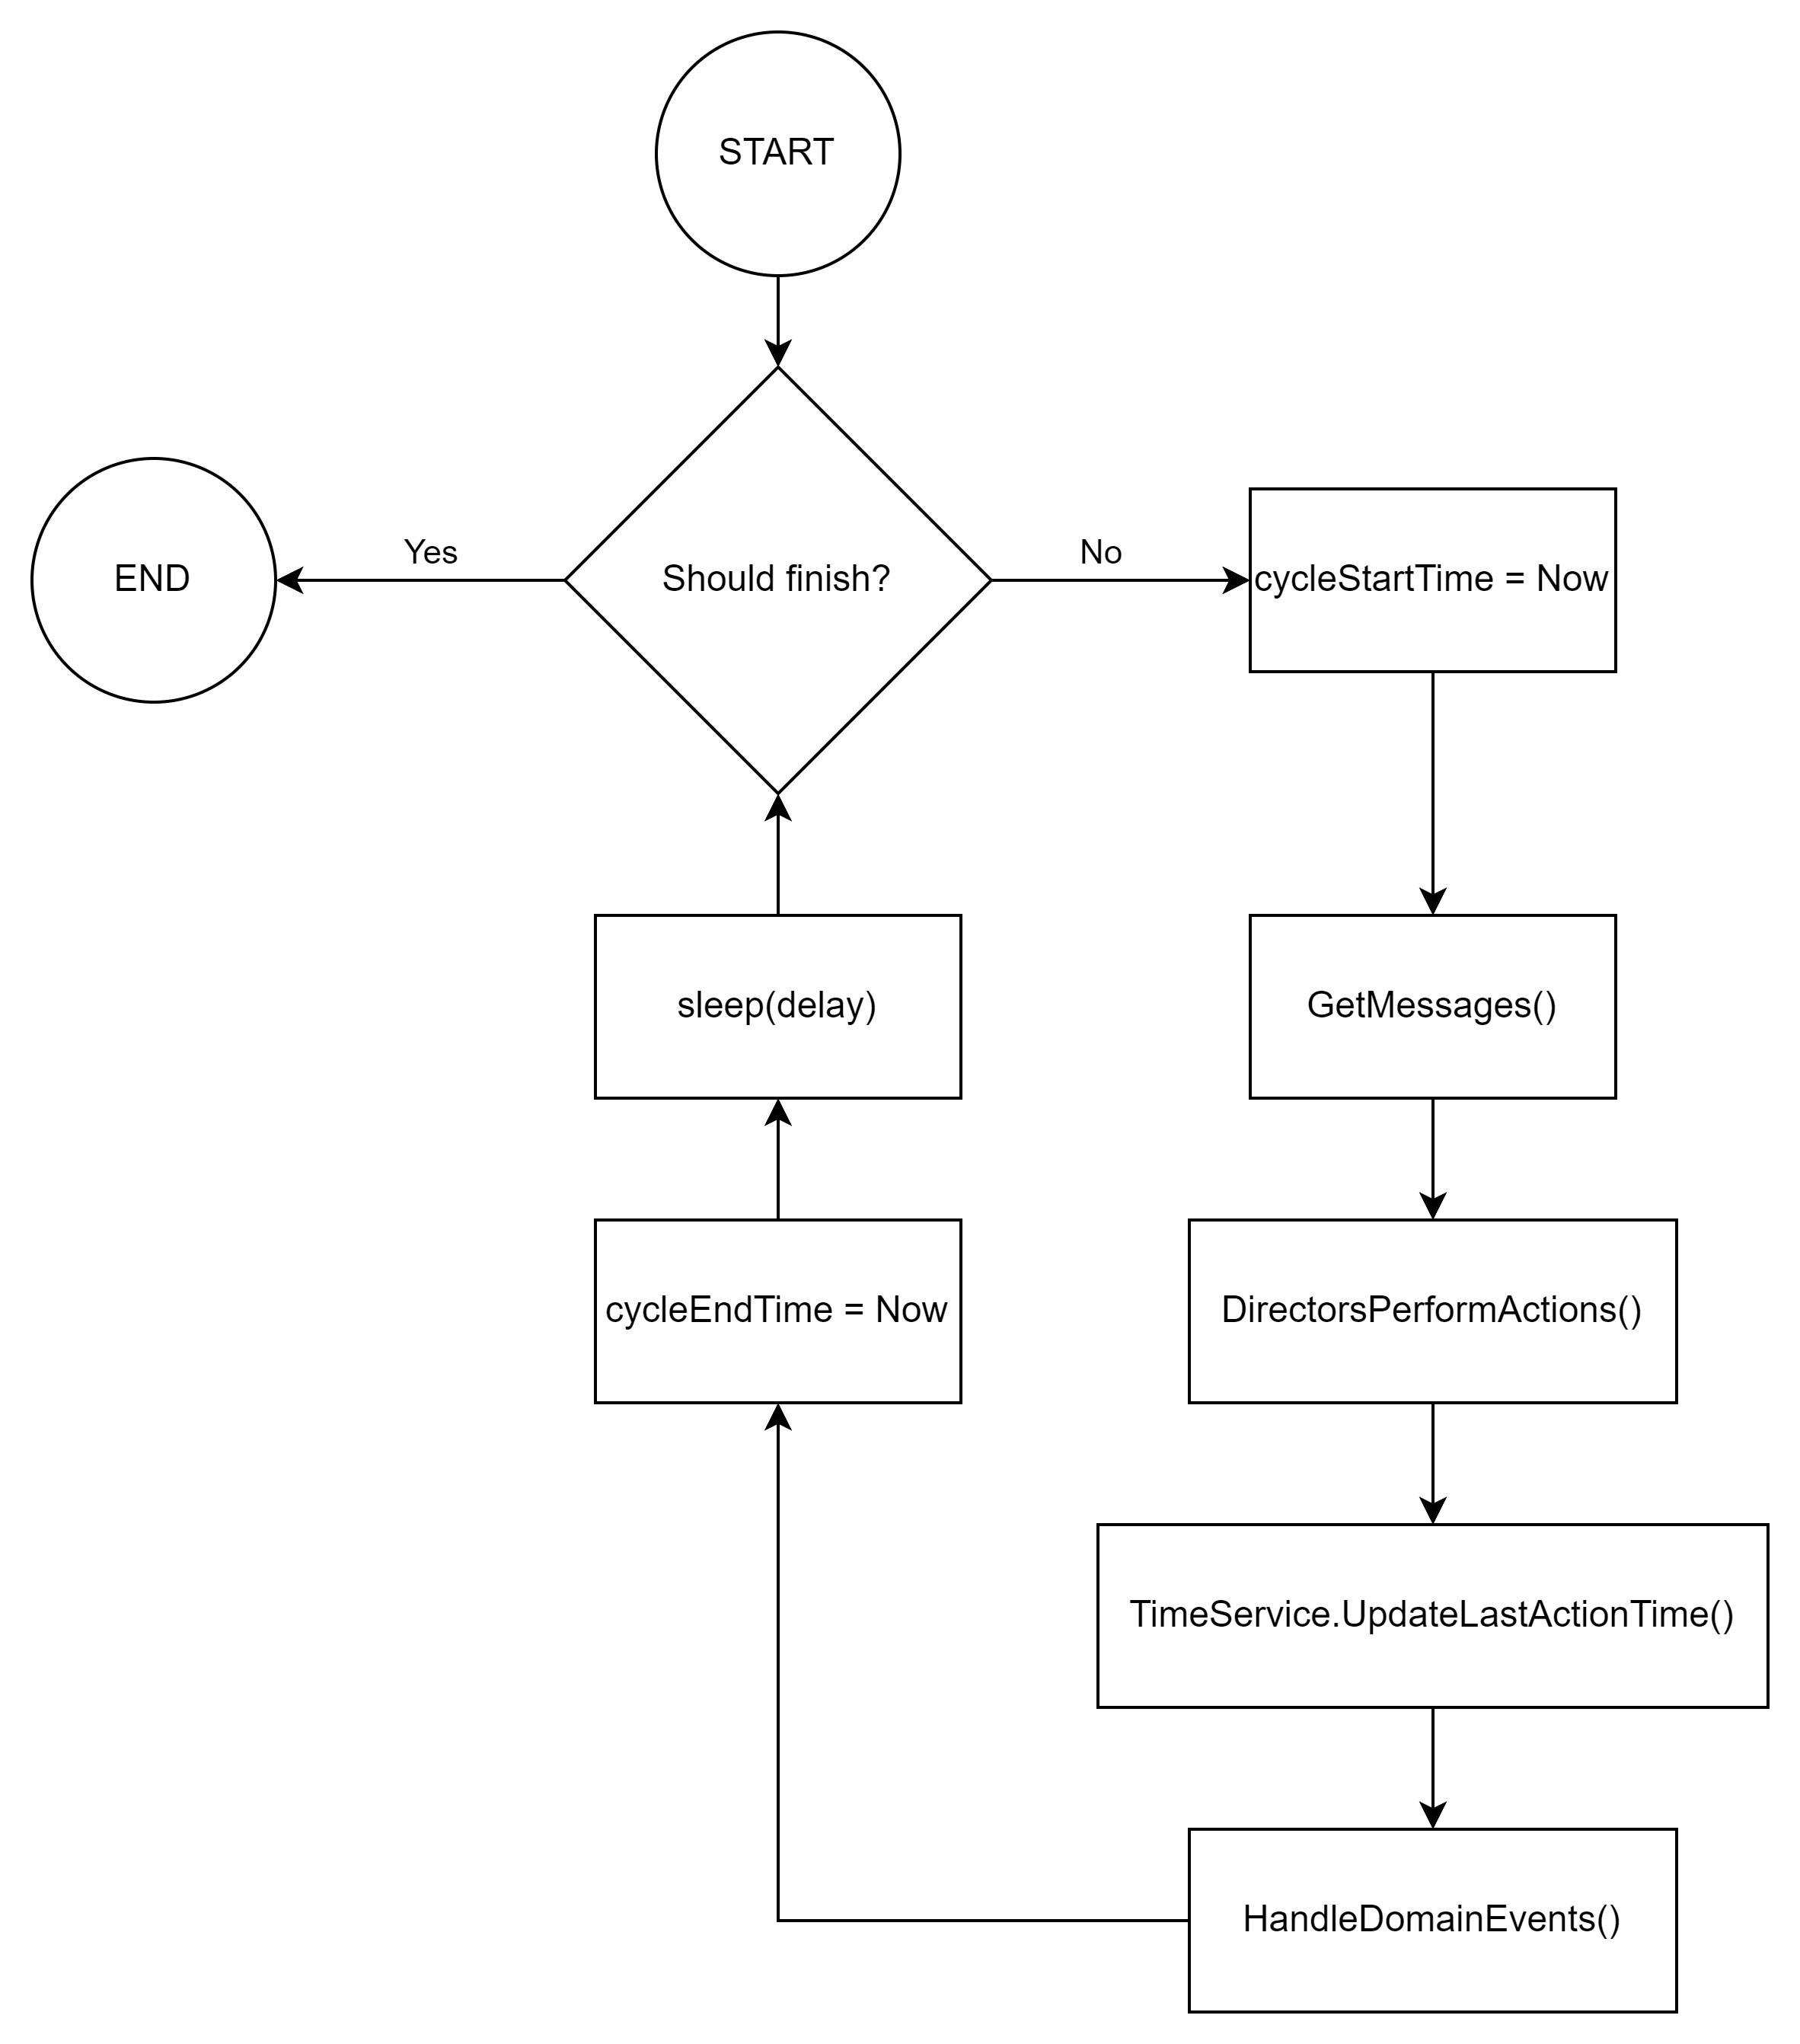
\includegraphics[width=\linewidth]{Simulation - Main Loop}
    \caption{Główna pętla symulacji}
    \label{fig:simulationMainLoop}
    \source{Opracowanie Własne}
\end{figure}

\par Pierwszy z nich odpowiada za generowanie, zarządzanie i przebieg incydentów w mieście. Zgodnie ze swoją konfiguracją, opisaną dokładniej w podrozdziale \ref{sec:konfiguracja}, potrafi tworzyć wydarzenia, jak i pisać ich scenariusze. Po rozpoczęciu danego zdarzenia, oczekuje on na odpowiedź ze strony patrolu, przybycie na miejsce, a następnie przeprowadza przebieg tego wydarzenia, zgodnie z wygenerowanym scenariuszem. Diagram \ref{fig:simulationIncidentLifecycle} przedstawia możliwe zmiany stanów incydentów.

\begin{figure}
    \centering
    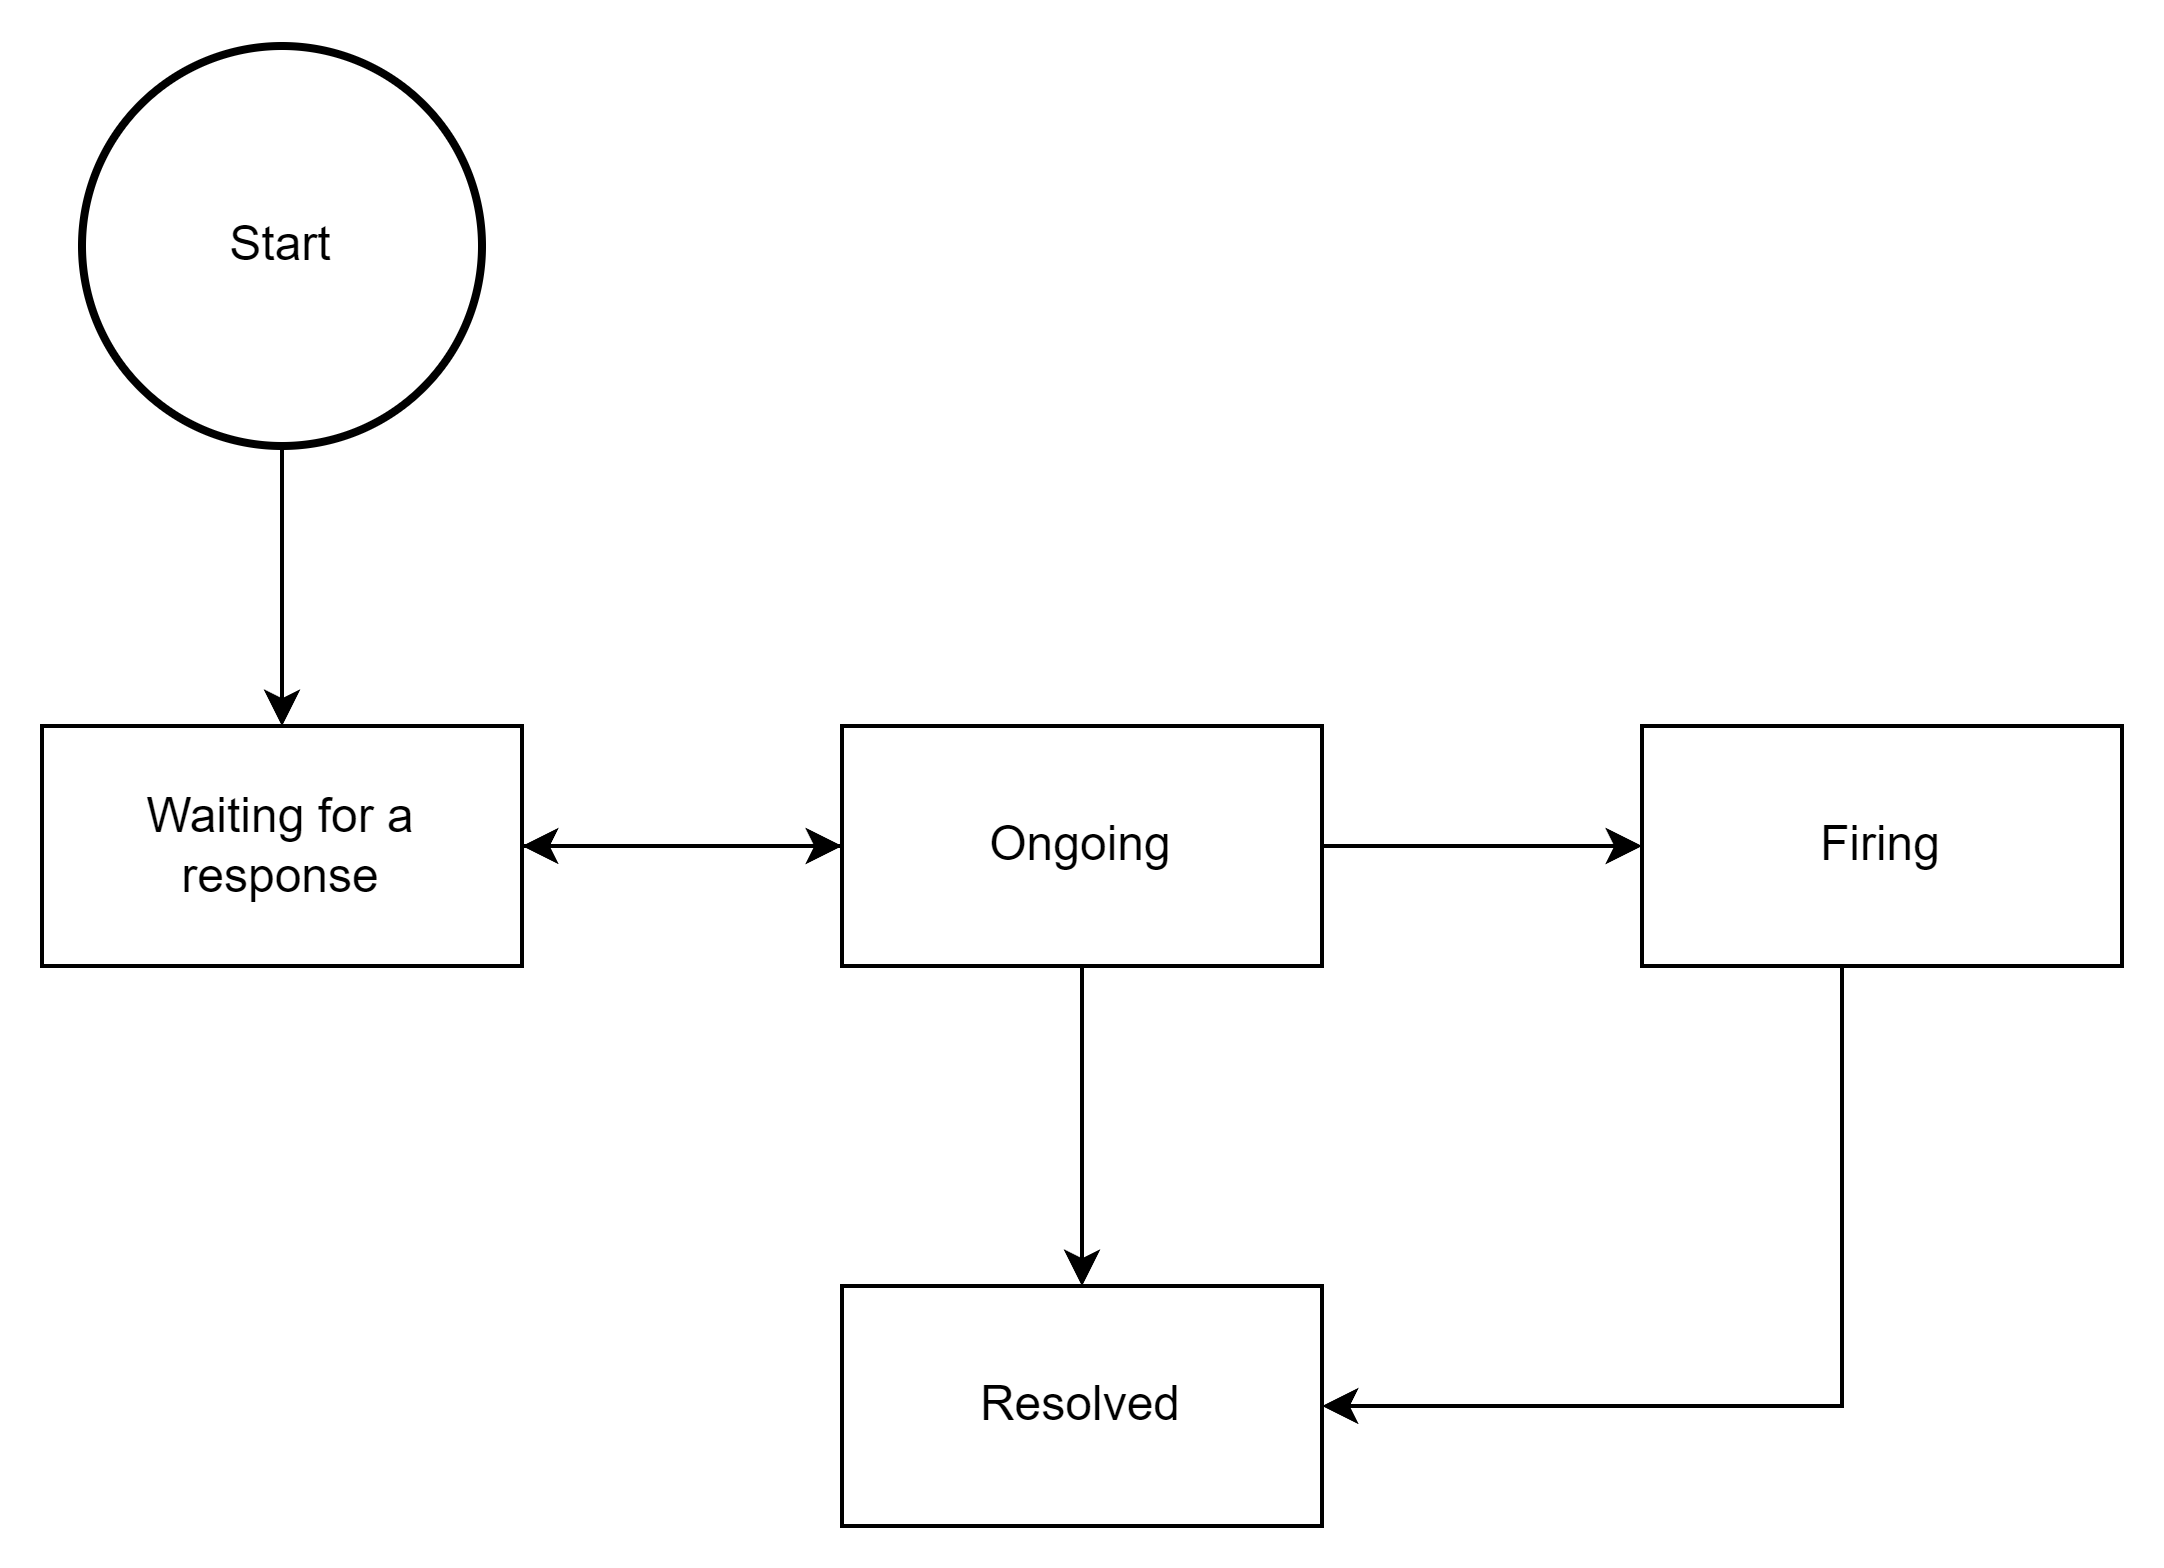
\includegraphics[width=\linewidth]{Incident - Lifecycle}
    \caption{Cykl życia incydentu}
    \label{fig:simulationIncidentLifecycle}
    \source{Opracowanie Własne}
\end{figure}

\par Zadaniem \texttt{PatrolDirector}a jest z kolei zarządzanie jednostkami policji. To on oblicza ich trasy, zarządza obecnie wykonywaną akcją, jak i przemieszcza te jednostki po mieście, według ściśle określonej logiki, która jest w pewnym stopniu konfigurowalna, zgodnie z opisem w podrozdziale \ref{sec:konfiguracja}.

\par Wszystkie zmiany, które zostaną dokonane na obiektach domenowych, automatycznie tworzą w nich tak zwane zdarzenia domenowe\english{Domain Event}. Są one następnie publikowane do zainteresowanych nimi odbiorców. Fragment \texttt{HandleDomainEvents()} przedstawiony na diagramie \ref{fig:simulationMainLoop}.